
% Default to the notebook output style

    


% Inherit from the specified cell style.




    
\documentclass[11pt]{article}

    
    
    \usepackage[T1]{fontenc}
    % Nicer default font (+ math font) than Computer Modern for most use cases
    \usepackage{mathpazo}

    % Basic figure setup, for now with no caption control since it's done
    % automatically by Pandoc (which extracts ![](path) syntax from Markdown).
    \usepackage{graphicx}
    % We will generate all images so they have a width \maxwidth. This means
    % that they will get their normal width if they fit onto the page, but
    % are scaled down if they would overflow the margins.
    \makeatletter
    \def\maxwidth{\ifdim\Gin@nat@width>\linewidth\linewidth
    \else\Gin@nat@width\fi}
    \makeatother
    \let\Oldincludegraphics\includegraphics
    % Set max figure width to be 80% of text width, for now hardcoded.
    \renewcommand{\includegraphics}[1]{\Oldincludegraphics[width=.8\maxwidth]{#1}}
    % Ensure that by default, figures have no caption (until we provide a
    % proper Figure object with a Caption API and a way to capture that
    % in the conversion process - todo).
    \usepackage{caption}
    \DeclareCaptionLabelFormat{nolabel}{}
    \captionsetup{labelformat=nolabel}

    \usepackage{adjustbox} % Used to constrain images to a maximum size 
    \usepackage{xcolor} % Allow colors to be defined
    \usepackage{enumerate} % Needed for markdown enumerations to work
    \usepackage{geometry} % Used to adjust the document margins
    \usepackage{amsmath} % Equations
    \usepackage{amssymb} % Equations
    \usepackage{textcomp} % defines textquotesingle
    % Hack from http://tex.stackexchange.com/a/47451/13684:
    \AtBeginDocument{%
        \def\PYZsq{\textquotesingle}% Upright quotes in Pygmentized code
    }
    \usepackage{upquote} % Upright quotes for verbatim code
    \usepackage{eurosym} % defines \euro
    \usepackage[mathletters]{ucs} % Extended unicode (utf-8) support
    \usepackage[utf8x]{inputenc} % Allow utf-8 characters in the tex document
    \usepackage{fancyvrb} % verbatim replacement that allows latex
    \usepackage{grffile} % extends the file name processing of package graphics 
                         % to support a larger range 
    % The hyperref package gives us a pdf with properly built
    % internal navigation ('pdf bookmarks' for the table of contents,
    % internal cross-reference links, web links for URLs, etc.)
    \usepackage{hyperref}
    \usepackage{longtable} % longtable support required by pandoc >1.10
    \usepackage{booktabs}  % table support for pandoc > 1.12.2
    \usepackage[inline]{enumitem} % IRkernel/repr support (it uses the enumerate* environment)
    \usepackage[normalem]{ulem} % ulem is needed to support strikethroughs (\sout)
                                % normalem makes italics be italics, not underlines
    

    
    
    % Colors for the hyperref package
    \definecolor{urlcolor}{rgb}{0,.145,.698}
    \definecolor{linkcolor}{rgb}{.71,0.21,0.01}
    \definecolor{citecolor}{rgb}{.12,.54,.11}

    % ANSI colors
    \definecolor{ansi-black}{HTML}{3E424D}
    \definecolor{ansi-black-intense}{HTML}{282C36}
    \definecolor{ansi-red}{HTML}{E75C58}
    \definecolor{ansi-red-intense}{HTML}{B22B31}
    \definecolor{ansi-green}{HTML}{00A250}
    \definecolor{ansi-green-intense}{HTML}{007427}
    \definecolor{ansi-yellow}{HTML}{DDB62B}
    \definecolor{ansi-yellow-intense}{HTML}{B27D12}
    \definecolor{ansi-blue}{HTML}{208FFB}
    \definecolor{ansi-blue-intense}{HTML}{0065CA}
    \definecolor{ansi-magenta}{HTML}{D160C4}
    \definecolor{ansi-magenta-intense}{HTML}{A03196}
    \definecolor{ansi-cyan}{HTML}{60C6C8}
    \definecolor{ansi-cyan-intense}{HTML}{258F8F}
    \definecolor{ansi-white}{HTML}{C5C1B4}
    \definecolor{ansi-white-intense}{HTML}{A1A6B2}

    % commands and environments needed by pandoc snippets
    % extracted from the output of `pandoc -s`
    \providecommand{\tightlist}{%
      \setlength{\itemsep}{0pt}\setlength{\parskip}{0pt}}
    \DefineVerbatimEnvironment{Highlighting}{Verbatim}{commandchars=\\\{\}}
    % Add ',fontsize=\small' for more characters per line
    \newenvironment{Shaded}{}{}
    \newcommand{\KeywordTok}[1]{\textcolor[rgb]{0.00,0.44,0.13}{\textbf{{#1}}}}
    \newcommand{\DataTypeTok}[1]{\textcolor[rgb]{0.56,0.13,0.00}{{#1}}}
    \newcommand{\DecValTok}[1]{\textcolor[rgb]{0.25,0.63,0.44}{{#1}}}
    \newcommand{\BaseNTok}[1]{\textcolor[rgb]{0.25,0.63,0.44}{{#1}}}
    \newcommand{\FloatTok}[1]{\textcolor[rgb]{0.25,0.63,0.44}{{#1}}}
    \newcommand{\CharTok}[1]{\textcolor[rgb]{0.25,0.44,0.63}{{#1}}}
    \newcommand{\StringTok}[1]{\textcolor[rgb]{0.25,0.44,0.63}{{#1}}}
    \newcommand{\CommentTok}[1]{\textcolor[rgb]{0.38,0.63,0.69}{\textit{{#1}}}}
    \newcommand{\OtherTok}[1]{\textcolor[rgb]{0.00,0.44,0.13}{{#1}}}
    \newcommand{\AlertTok}[1]{\textcolor[rgb]{1.00,0.00,0.00}{\textbf{{#1}}}}
    \newcommand{\FunctionTok}[1]{\textcolor[rgb]{0.02,0.16,0.49}{{#1}}}
    \newcommand{\RegionMarkerTok}[1]{{#1}}
    \newcommand{\ErrorTok}[1]{\textcolor[rgb]{1.00,0.00,0.00}{\textbf{{#1}}}}
    \newcommand{\NormalTok}[1]{{#1}}
    
    % Additional commands for more recent versions of Pandoc
    \newcommand{\ConstantTok}[1]{\textcolor[rgb]{0.53,0.00,0.00}{{#1}}}
    \newcommand{\SpecialCharTok}[1]{\textcolor[rgb]{0.25,0.44,0.63}{{#1}}}
    \newcommand{\VerbatimStringTok}[1]{\textcolor[rgb]{0.25,0.44,0.63}{{#1}}}
    \newcommand{\SpecialStringTok}[1]{\textcolor[rgb]{0.73,0.40,0.53}{{#1}}}
    \newcommand{\ImportTok}[1]{{#1}}
    \newcommand{\DocumentationTok}[1]{\textcolor[rgb]{0.73,0.13,0.13}{\textit{{#1}}}}
    \newcommand{\AnnotationTok}[1]{\textcolor[rgb]{0.38,0.63,0.69}{\textbf{\textit{{#1}}}}}
    \newcommand{\CommentVarTok}[1]{\textcolor[rgb]{0.38,0.63,0.69}{\textbf{\textit{{#1}}}}}
    \newcommand{\VariableTok}[1]{\textcolor[rgb]{0.10,0.09,0.49}{{#1}}}
    \newcommand{\ControlFlowTok}[1]{\textcolor[rgb]{0.00,0.44,0.13}{\textbf{{#1}}}}
    \newcommand{\OperatorTok}[1]{\textcolor[rgb]{0.40,0.40,0.40}{{#1}}}
    \newcommand{\BuiltInTok}[1]{{#1}}
    \newcommand{\ExtensionTok}[1]{{#1}}
    \newcommand{\PreprocessorTok}[1]{\textcolor[rgb]{0.74,0.48,0.00}{{#1}}}
    \newcommand{\AttributeTok}[1]{\textcolor[rgb]{0.49,0.56,0.16}{{#1}}}
    \newcommand{\InformationTok}[1]{\textcolor[rgb]{0.38,0.63,0.69}{\textbf{\textit{{#1}}}}}
    \newcommand{\WarningTok}[1]{\textcolor[rgb]{0.38,0.63,0.69}{\textbf{\textit{{#1}}}}}
    
    
    % Define a nice break command that doesn't care if a line doesn't already
    % exist.
    \def\br{\hspace*{\fill} \\* }
    % Math Jax compatability definitions
    \def\gt{>}
    \def\lt{<}
    % Document parameters
    \title{LIME\_InceptionV3}
    
    
    

    % Pygments definitions
    
\makeatletter
\def\PY@reset{\let\PY@it=\relax \let\PY@bf=\relax%
    \let\PY@ul=\relax \let\PY@tc=\relax%
    \let\PY@bc=\relax \let\PY@ff=\relax}
\def\PY@tok#1{\csname PY@tok@#1\endcsname}
\def\PY@toks#1+{\ifx\relax#1\empty\else%
    \PY@tok{#1}\expandafter\PY@toks\fi}
\def\PY@do#1{\PY@bc{\PY@tc{\PY@ul{%
    \PY@it{\PY@bf{\PY@ff{#1}}}}}}}
\def\PY#1#2{\PY@reset\PY@toks#1+\relax+\PY@do{#2}}

\expandafter\def\csname PY@tok@w\endcsname{\def\PY@tc##1{\textcolor[rgb]{0.73,0.73,0.73}{##1}}}
\expandafter\def\csname PY@tok@c\endcsname{\let\PY@it=\textit\def\PY@tc##1{\textcolor[rgb]{0.25,0.50,0.50}{##1}}}
\expandafter\def\csname PY@tok@cp\endcsname{\def\PY@tc##1{\textcolor[rgb]{0.74,0.48,0.00}{##1}}}
\expandafter\def\csname PY@tok@k\endcsname{\let\PY@bf=\textbf\def\PY@tc##1{\textcolor[rgb]{0.00,0.50,0.00}{##1}}}
\expandafter\def\csname PY@tok@kp\endcsname{\def\PY@tc##1{\textcolor[rgb]{0.00,0.50,0.00}{##1}}}
\expandafter\def\csname PY@tok@kt\endcsname{\def\PY@tc##1{\textcolor[rgb]{0.69,0.00,0.25}{##1}}}
\expandafter\def\csname PY@tok@o\endcsname{\def\PY@tc##1{\textcolor[rgb]{0.40,0.40,0.40}{##1}}}
\expandafter\def\csname PY@tok@ow\endcsname{\let\PY@bf=\textbf\def\PY@tc##1{\textcolor[rgb]{0.67,0.13,1.00}{##1}}}
\expandafter\def\csname PY@tok@nb\endcsname{\def\PY@tc##1{\textcolor[rgb]{0.00,0.50,0.00}{##1}}}
\expandafter\def\csname PY@tok@nf\endcsname{\def\PY@tc##1{\textcolor[rgb]{0.00,0.00,1.00}{##1}}}
\expandafter\def\csname PY@tok@nc\endcsname{\let\PY@bf=\textbf\def\PY@tc##1{\textcolor[rgb]{0.00,0.00,1.00}{##1}}}
\expandafter\def\csname PY@tok@nn\endcsname{\let\PY@bf=\textbf\def\PY@tc##1{\textcolor[rgb]{0.00,0.00,1.00}{##1}}}
\expandafter\def\csname PY@tok@ne\endcsname{\let\PY@bf=\textbf\def\PY@tc##1{\textcolor[rgb]{0.82,0.25,0.23}{##1}}}
\expandafter\def\csname PY@tok@nv\endcsname{\def\PY@tc##1{\textcolor[rgb]{0.10,0.09,0.49}{##1}}}
\expandafter\def\csname PY@tok@no\endcsname{\def\PY@tc##1{\textcolor[rgb]{0.53,0.00,0.00}{##1}}}
\expandafter\def\csname PY@tok@nl\endcsname{\def\PY@tc##1{\textcolor[rgb]{0.63,0.63,0.00}{##1}}}
\expandafter\def\csname PY@tok@ni\endcsname{\let\PY@bf=\textbf\def\PY@tc##1{\textcolor[rgb]{0.60,0.60,0.60}{##1}}}
\expandafter\def\csname PY@tok@na\endcsname{\def\PY@tc##1{\textcolor[rgb]{0.49,0.56,0.16}{##1}}}
\expandafter\def\csname PY@tok@nt\endcsname{\let\PY@bf=\textbf\def\PY@tc##1{\textcolor[rgb]{0.00,0.50,0.00}{##1}}}
\expandafter\def\csname PY@tok@nd\endcsname{\def\PY@tc##1{\textcolor[rgb]{0.67,0.13,1.00}{##1}}}
\expandafter\def\csname PY@tok@s\endcsname{\def\PY@tc##1{\textcolor[rgb]{0.73,0.13,0.13}{##1}}}
\expandafter\def\csname PY@tok@sd\endcsname{\let\PY@it=\textit\def\PY@tc##1{\textcolor[rgb]{0.73,0.13,0.13}{##1}}}
\expandafter\def\csname PY@tok@si\endcsname{\let\PY@bf=\textbf\def\PY@tc##1{\textcolor[rgb]{0.73,0.40,0.53}{##1}}}
\expandafter\def\csname PY@tok@se\endcsname{\let\PY@bf=\textbf\def\PY@tc##1{\textcolor[rgb]{0.73,0.40,0.13}{##1}}}
\expandafter\def\csname PY@tok@sr\endcsname{\def\PY@tc##1{\textcolor[rgb]{0.73,0.40,0.53}{##1}}}
\expandafter\def\csname PY@tok@ss\endcsname{\def\PY@tc##1{\textcolor[rgb]{0.10,0.09,0.49}{##1}}}
\expandafter\def\csname PY@tok@sx\endcsname{\def\PY@tc##1{\textcolor[rgb]{0.00,0.50,0.00}{##1}}}
\expandafter\def\csname PY@tok@m\endcsname{\def\PY@tc##1{\textcolor[rgb]{0.40,0.40,0.40}{##1}}}
\expandafter\def\csname PY@tok@gh\endcsname{\let\PY@bf=\textbf\def\PY@tc##1{\textcolor[rgb]{0.00,0.00,0.50}{##1}}}
\expandafter\def\csname PY@tok@gu\endcsname{\let\PY@bf=\textbf\def\PY@tc##1{\textcolor[rgb]{0.50,0.00,0.50}{##1}}}
\expandafter\def\csname PY@tok@gd\endcsname{\def\PY@tc##1{\textcolor[rgb]{0.63,0.00,0.00}{##1}}}
\expandafter\def\csname PY@tok@gi\endcsname{\def\PY@tc##1{\textcolor[rgb]{0.00,0.63,0.00}{##1}}}
\expandafter\def\csname PY@tok@gr\endcsname{\def\PY@tc##1{\textcolor[rgb]{1.00,0.00,0.00}{##1}}}
\expandafter\def\csname PY@tok@ge\endcsname{\let\PY@it=\textit}
\expandafter\def\csname PY@tok@gs\endcsname{\let\PY@bf=\textbf}
\expandafter\def\csname PY@tok@gp\endcsname{\let\PY@bf=\textbf\def\PY@tc##1{\textcolor[rgb]{0.00,0.00,0.50}{##1}}}
\expandafter\def\csname PY@tok@go\endcsname{\def\PY@tc##1{\textcolor[rgb]{0.53,0.53,0.53}{##1}}}
\expandafter\def\csname PY@tok@gt\endcsname{\def\PY@tc##1{\textcolor[rgb]{0.00,0.27,0.87}{##1}}}
\expandafter\def\csname PY@tok@err\endcsname{\def\PY@bc##1{\setlength{\fboxsep}{0pt}\fcolorbox[rgb]{1.00,0.00,0.00}{1,1,1}{\strut ##1}}}
\expandafter\def\csname PY@tok@kc\endcsname{\let\PY@bf=\textbf\def\PY@tc##1{\textcolor[rgb]{0.00,0.50,0.00}{##1}}}
\expandafter\def\csname PY@tok@kd\endcsname{\let\PY@bf=\textbf\def\PY@tc##1{\textcolor[rgb]{0.00,0.50,0.00}{##1}}}
\expandafter\def\csname PY@tok@kn\endcsname{\let\PY@bf=\textbf\def\PY@tc##1{\textcolor[rgb]{0.00,0.50,0.00}{##1}}}
\expandafter\def\csname PY@tok@kr\endcsname{\let\PY@bf=\textbf\def\PY@tc##1{\textcolor[rgb]{0.00,0.50,0.00}{##1}}}
\expandafter\def\csname PY@tok@bp\endcsname{\def\PY@tc##1{\textcolor[rgb]{0.00,0.50,0.00}{##1}}}
\expandafter\def\csname PY@tok@fm\endcsname{\def\PY@tc##1{\textcolor[rgb]{0.00,0.00,1.00}{##1}}}
\expandafter\def\csname PY@tok@vc\endcsname{\def\PY@tc##1{\textcolor[rgb]{0.10,0.09,0.49}{##1}}}
\expandafter\def\csname PY@tok@vg\endcsname{\def\PY@tc##1{\textcolor[rgb]{0.10,0.09,0.49}{##1}}}
\expandafter\def\csname PY@tok@vi\endcsname{\def\PY@tc##1{\textcolor[rgb]{0.10,0.09,0.49}{##1}}}
\expandafter\def\csname PY@tok@vm\endcsname{\def\PY@tc##1{\textcolor[rgb]{0.10,0.09,0.49}{##1}}}
\expandafter\def\csname PY@tok@sa\endcsname{\def\PY@tc##1{\textcolor[rgb]{0.73,0.13,0.13}{##1}}}
\expandafter\def\csname PY@tok@sb\endcsname{\def\PY@tc##1{\textcolor[rgb]{0.73,0.13,0.13}{##1}}}
\expandafter\def\csname PY@tok@sc\endcsname{\def\PY@tc##1{\textcolor[rgb]{0.73,0.13,0.13}{##1}}}
\expandafter\def\csname PY@tok@dl\endcsname{\def\PY@tc##1{\textcolor[rgb]{0.73,0.13,0.13}{##1}}}
\expandafter\def\csname PY@tok@s2\endcsname{\def\PY@tc##1{\textcolor[rgb]{0.73,0.13,0.13}{##1}}}
\expandafter\def\csname PY@tok@sh\endcsname{\def\PY@tc##1{\textcolor[rgb]{0.73,0.13,0.13}{##1}}}
\expandafter\def\csname PY@tok@s1\endcsname{\def\PY@tc##1{\textcolor[rgb]{0.73,0.13,0.13}{##1}}}
\expandafter\def\csname PY@tok@mb\endcsname{\def\PY@tc##1{\textcolor[rgb]{0.40,0.40,0.40}{##1}}}
\expandafter\def\csname PY@tok@mf\endcsname{\def\PY@tc##1{\textcolor[rgb]{0.40,0.40,0.40}{##1}}}
\expandafter\def\csname PY@tok@mh\endcsname{\def\PY@tc##1{\textcolor[rgb]{0.40,0.40,0.40}{##1}}}
\expandafter\def\csname PY@tok@mi\endcsname{\def\PY@tc##1{\textcolor[rgb]{0.40,0.40,0.40}{##1}}}
\expandafter\def\csname PY@tok@il\endcsname{\def\PY@tc##1{\textcolor[rgb]{0.40,0.40,0.40}{##1}}}
\expandafter\def\csname PY@tok@mo\endcsname{\def\PY@tc##1{\textcolor[rgb]{0.40,0.40,0.40}{##1}}}
\expandafter\def\csname PY@tok@ch\endcsname{\let\PY@it=\textit\def\PY@tc##1{\textcolor[rgb]{0.25,0.50,0.50}{##1}}}
\expandafter\def\csname PY@tok@cm\endcsname{\let\PY@it=\textit\def\PY@tc##1{\textcolor[rgb]{0.25,0.50,0.50}{##1}}}
\expandafter\def\csname PY@tok@cpf\endcsname{\let\PY@it=\textit\def\PY@tc##1{\textcolor[rgb]{0.25,0.50,0.50}{##1}}}
\expandafter\def\csname PY@tok@c1\endcsname{\let\PY@it=\textit\def\PY@tc##1{\textcolor[rgb]{0.25,0.50,0.50}{##1}}}
\expandafter\def\csname PY@tok@cs\endcsname{\let\PY@it=\textit\def\PY@tc##1{\textcolor[rgb]{0.25,0.50,0.50}{##1}}}

\def\PYZbs{\char`\\}
\def\PYZus{\char`\_}
\def\PYZob{\char`\{}
\def\PYZcb{\char`\}}
\def\PYZca{\char`\^}
\def\PYZam{\char`\&}
\def\PYZlt{\char`\<}
\def\PYZgt{\char`\>}
\def\PYZsh{\char`\#}
\def\PYZpc{\char`\%}
\def\PYZdl{\char`\$}
\def\PYZhy{\char`\-}
\def\PYZsq{\char`\'}
\def\PYZdq{\char`\"}
\def\PYZti{\char`\~}
% for compatibility with earlier versions
\def\PYZat{@}
\def\PYZlb{[}
\def\PYZrb{]}
\makeatother


    % Exact colors from NB
    \definecolor{incolor}{rgb}{0.0, 0.0, 0.5}
    \definecolor{outcolor}{rgb}{0.545, 0.0, 0.0}



    
    % Prevent overflowing lines due to hard-to-break entities
    \sloppy 
    % Setup hyperref package
    \hypersetup{
      breaklinks=true,  % so long urls are correctly broken across lines
      colorlinks=true,
      urlcolor=urlcolor,
      linkcolor=linkcolor,
      citecolor=citecolor,
      }
    % Slightly bigger margins than the latex defaults
    
    \geometry{verbose,tmargin=1in,bmargin=1in,lmargin=1in,rmargin=1in}
    
    

    \begin{document}
    
    
    \maketitle
    
    

    
    \section{Explainable Artificial Intelligence
(xAI)}\label{explainable-artificial-intelligence-xai}

    \subsection{Background}\label{background}

\begin{itemize}
\tightlist
\item
  Success stories of AI in diverse applications(i.e. Autonomous Driving,
  Manufacturing, Game, Medical..)
\item
  Limitations : Inability to \emph{explain} the model's thoughts
\item
  Importance of Explainability
\end{itemize}

\begin{enumerate}
\def\labelenumi{\arabic{enumi}.}
\tightlist
\item
  Validation
\item
  Trustness
\item
  Legal Compliances
\end{enumerate}

    \subsection{What we are trying to do?}\label{what-we-are-trying-to-do}

\begin{itemize}
\tightlist
\item
  Presents a novel method to generate explanations for AI machines
\end{itemize}

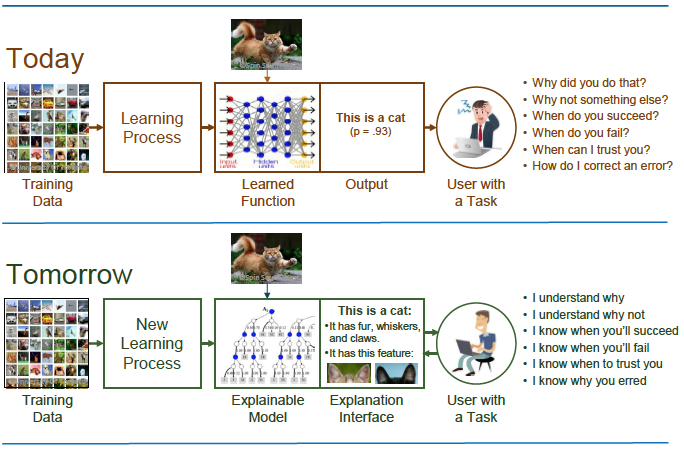
\includegraphics{xAI_Intro.png}

\begin{verbatim}
<center>Source : *Gunning 2016, Explainable Artificial Intelligence, DARPA* </center>
\end{verbatim}

    \subsection{Demo : Highlighting spatio attention of an image by
LIME}\label{demo-highlighting-spatio-attention-of-an-image-by-lime}

\subsubsection{(LIME : Local Interpretable Model-agnostic
Explanation)}\label{lime-local-interpretable-model-agnostic-explanation}

    \begin{Verbatim}[commandchars=\\\{\}]
{\color{incolor}In [{\color{incolor}2}]:} \PY{k+kn}{import} \PY{n+nn}{os}
        \PY{k+kn}{import} \PY{n+nn}{keras}
        \PY{k+kn}{from} \PY{n+nn}{keras}\PY{n+nn}{.}\PY{n+nn}{applications} \PY{k}{import} \PY{n}{inception\PYZus{}resnet\PYZus{}v2}
        \PY{k+kn}{from} \PY{n+nn}{keras}\PY{n+nn}{.}\PY{n+nn}{applications}\PY{n+nn}{.}\PY{n+nn}{inception\PYZus{}resnet\PYZus{}v2} \PY{k}{import} \PY{n}{InceptionResNetV2}
        \PY{k+kn}{from} \PY{n+nn}{keras}\PY{n+nn}{.}\PY{n+nn}{applications}\PY{n+nn}{.}\PY{n+nn}{inception\PYZus{}resnet\PYZus{}v2} \PY{k}{import} \PY{n}{preprocess\PYZus{}input}
        \PY{k+kn}{from} \PY{n+nn}{keras}\PY{n+nn}{.}\PY{n+nn}{applications}\PY{n+nn}{.}\PY{n+nn}{inception\PYZus{}resnet\PYZus{}v2} \PY{k}{import} \PY{n}{decode\PYZus{}predictions}
        
        \PY{k+kn}{from} \PY{n+nn}{keras}\PY{n+nn}{.}\PY{n+nn}{preprocessing}\PY{n+nn}{.}\PY{n+nn}{image} \PY{k}{import} \PY{n}{ImageDataGenerator}\PY{p}{,} \PY{n}{array\PYZus{}to\PYZus{}img}\PY{p}{,} \PY{n}{img\PYZus{}to\PYZus{}array}\PY{p}{,} \PY{n}{load\PYZus{}img}
        
        \PY{k+kn}{from} \PY{n+nn}{keras}\PY{n+nn}{.}\PY{n+nn}{models} \PY{k}{import} \PY{n}{Model}
        \PY{k+kn}{from} \PY{n+nn}{keras}\PY{n+nn}{.}\PY{n+nn}{layers} \PY{k}{import} \PY{n}{Dense}\PY{p}{,} \PY{n}{GlobalAveragePooling2D}
        \PY{k+kn}{from} \PY{n+nn}{keras} \PY{k}{import} \PY{n}{backend} \PY{k}{as} \PY{n}{K}
        \PY{k+kn}{from} \PY{n+nn}{skimage}\PY{n+nn}{.}\PY{n+nn}{io} \PY{k}{import} \PY{n}{imread}
        
        \PY{k+kn}{import} \PY{n+nn}{matplotlib}\PY{n+nn}{.}\PY{n+nn}{pyplot} \PY{k}{as} \PY{n+nn}{plt}
        \PY{k+kn}{import} \PY{n+nn}{numpy} \PY{k}{as} \PY{n+nn}{np}
        \PY{o}{\PYZpc{}}\PY{k}{matplotlib} inline
        \PY{n+nb}{print}\PY{p}{(}\PY{l+s+s1}{\PYZsq{}}\PY{l+s+s1}{Notebook run using keras:}\PY{l+s+s1}{\PYZsq{}}\PY{p}{,} \PY{n}{keras}\PY{o}{.}\PY{n}{\PYZus{}\PYZus{}version\PYZus{}\PYZus{}}\PY{p}{)}
\end{Verbatim}


    \begin{Verbatim}[commandchars=\\\{\}]
Using TensorFlow backend.

    \end{Verbatim}

    \begin{Verbatim}[commandchars=\\\{\}]
Notebook run using keras: 2.2.4

    \end{Verbatim}

    \subsubsection{Using InceptionResNetV2 Model as a object detection
model}\label{using-inceptionresnetv2-model-as-a-object-detection-model}

    \begin{Verbatim}[commandchars=\\\{\}]
{\color{incolor}In [{\color{incolor}4}]:} \PY{c+c1}{\PYZsh{} create the base pre\PYZhy{}trained model}
        \PY{n}{base\PYZus{}model} \PY{o}{=} \PY{n}{InceptionResNetV2}\PY{p}{(}\PY{n}{weights}\PY{o}{=}\PY{l+s+s1}{\PYZsq{}}\PY{l+s+s1}{imagenet}\PY{l+s+s1}{\PYZsq{}}\PY{p}{,} \PY{n}{include\PYZus{}top}\PY{o}{=}\PY{k+kc}{True}\PY{p}{)}
        \PY{c+c1}{\PYZsh{}base\PYZus{}model = VGG19(weights=\PYZsq{}imagenet\PYZsq{}, include\PYZus{}top=True)}
\end{Verbatim}


    \begin{Verbatim}[commandchars=\\\{\}]
{\color{incolor}In [{\color{incolor}5}]:} \PY{k}{def} \PY{n+nf}{transform\PYZus{}img\PYZus{}fn}\PY{p}{(}\PY{n}{path\PYZus{}list}\PY{p}{)}\PY{p}{:}
            \PY{n}{output} \PY{o}{=} \PY{p}{[}\PY{p}{]}
            \PY{k}{for} \PY{n}{img\PYZus{}path} \PY{o+ow}{in} \PY{n}{path\PYZus{}list}\PY{p}{:}
                \PY{n}{img} \PY{o}{=} \PY{n}{load\PYZus{}img}\PY{p}{(}\PY{n}{img\PYZus{}path}\PY{p}{,} \PY{n}{target\PYZus{}size}\PY{o}{=}\PY{p}{(}\PY{l+m+mi}{299}\PY{p}{,}\PY{l+m+mi}{299}\PY{p}{)}\PY{p}{)} \PY{c+c1}{\PYZsh{} For Inception\PYZus{}resnet\PYZus{}v2}
                \PY{c+c1}{\PYZsh{}img = load\PYZus{}img(img\PYZus{}path, target\PYZus{}size=(224,224)) \PYZsh{} For VGG19}
                
                \PY{n}{x} \PY{o}{=} \PY{n}{img\PYZus{}to\PYZus{}array}\PY{p}{(}\PY{n}{img}\PY{p}{)}  \PY{c+c1}{\PYZsh{} this is a Numpy array with shape (3(RGB), width, height)}
                \PY{n}{x} \PY{o}{=} \PY{n}{np}\PY{o}{.}\PY{n}{expand\PYZus{}dims}\PY{p}{(}\PY{n}{x}\PY{p}{,} \PY{n}{axis}\PY{o}{=}\PY{l+m+mi}{0}\PY{p}{)} \PY{c+c1}{\PYZsh{} this is a Numpy array with shape (1, 3(RGB), width, height)}
                \PY{n}{x} \PY{o}{=} \PY{n}{preprocess\PYZus{}input}\PY{p}{(}\PY{n}{x}\PY{p}{)}
                \PY{n}{output}\PY{o}{.}\PY{n}{append}\PY{p}{(}\PY{n}{x}\PY{p}{)}
            \PY{k}{return} \PY{n}{np}\PY{o}{.}\PY{n}{vstack}\PY{p}{(}\PY{n}{output}\PY{p}{)}
\end{Verbatim}


    \subsubsection{Sample images}\label{sample-images}

    \begin{Verbatim}[commandchars=\\\{\}]
{\color{incolor}In [{\color{incolor}46}]:} \PY{k+kn}{import} \PY{n+nn}{glob}
         
         \PY{n}{file\PYZus{}list} \PY{o}{=} \PY{n}{glob}\PY{o}{.}\PY{n}{glob}\PY{p}{(}\PY{l+s+s2}{\PYZdq{}}\PY{l+s+s2}{./Images/*/*}\PY{l+s+s2}{\PYZdq{}}\PY{p}{,} \PY{n}{recursive}\PY{o}{=}\PY{k+kc}{True}\PY{p}{)}
         \PY{n+nb}{print}\PY{p}{(}\PY{l+s+s1}{\PYZsq{}}\PY{l+s+s1}{Loading Images}\PY{l+s+s1}{\PYZsq{}}\PY{p}{)}
         \PY{c+c1}{\PYZsh{}print(\PYZsq{}Number of Images found : \PYZsq{}, len(file\PYZus{}list))}
         
         
         \PY{n}{file\PYZus{}list} \PY{o}{=} \PY{p}{[}\PY{n}{file\PYZus{}list}\PY{p}{[}\PY{n}{x}\PY{p}{]} \PY{k}{for} \PY{n}{x} \PY{o+ow}{in} \PY{p}{[}\PY{l+m+mi}{0}\PY{p}{,}\PY{l+m+mi}{3}\PY{p}{,}\PY{l+m+mi}{5}\PY{p}{]}\PY{p}{]} 
         \PY{n}{img\PYZus{}list} \PY{o}{=} \PY{n}{transform\PYZus{}img\PYZus{}fn}\PY{p}{(}\PY{n}{file\PYZus{}list}\PY{p}{)}
         \PY{c+c1}{\PYZsh{}img\PYZus{}list = [img\PYZus{}list[x] for x in [0,3,5]]}
         
         \PY{n}{fig} \PY{o}{=} \PY{n}{plt}\PY{o}{.}\PY{n}{figure}\PY{p}{(}\PY{p}{)}
         \PY{n}{fig}\PY{o}{.}\PY{n}{set\PYZus{}size\PYZus{}inches}\PY{p}{(}\PY{l+m+mi}{10}\PY{p}{,}\PY{l+m+mi}{10}\PY{p}{)}
         
         \PY{k}{for} \PY{n}{idx}\PY{p}{,} \PY{n}{img} \PY{o+ow}{in} \PY{n+nb}{enumerate}\PY{p}{(}\PY{n}{img\PYZus{}list}\PY{p}{)}\PY{p}{:}
             \PY{n}{ax} \PY{o}{=} \PY{n}{plt}\PY{o}{.}\PY{n}{subplot}\PY{p}{(}\PY{l+m+mi}{1}\PY{p}{,}\PY{l+m+mi}{3}\PY{p}{,}\PY{n}{idx}\PY{o}{+}\PY{l+m+mi}{1}\PY{p}{)}
             \PY{n}{ax}\PY{o}{.}\PY{n}{set\PYZus{}title}\PY{p}{(}\PY{n}{file\PYZus{}list}\PY{p}{[}\PY{n}{idx}\PY{p}{]}\PY{o}{.}\PY{n}{split}\PY{p}{(}\PY{l+s+s1}{\PYZsq{}}\PY{l+s+s1}{/}\PY{l+s+s1}{\PYZsq{}}\PY{p}{)}\PY{p}{[}\PY{l+m+mi}{2}\PY{p}{]}\PY{p}{)}
             \PY{n}{plt}\PY{o}{.}\PY{n}{axis}\PY{p}{(}\PY{l+s+s1}{\PYZsq{}}\PY{l+s+s1}{off}\PY{l+s+s1}{\PYZsq{}}\PY{p}{)}
             \PY{n}{plt}\PY{o}{.}\PY{n}{imshow}\PY{p}{(}\PY{n}{img\PYZus{}list}\PY{p}{[}\PY{n}{idx}\PY{p}{]} \PY{o}{/} \PY{l+m+mi}{2} \PY{o}{+} \PY{l+m+mf}{0.5}\PY{p}{)}
\end{Verbatim}


    \begin{Verbatim}[commandchars=\\\{\}]
Loading Images

    \end{Verbatim}

    \begin{center}
    \adjustimage{max size={0.9\linewidth}{0.9\paperheight}}{output_9_1.png}
    \end{center}
    { \hspace*{\fill} \\}
    
    \subsubsection{Do predict what the object is by
A.I.}\label{do-predict-what-the-object-is-by-a.i.}

    \begin{Verbatim}[commandchars=\\\{\}]
{\color{incolor}In [{\color{incolor}80}]:} \PY{c+c1}{\PYZsh{}preds = base\PYZus{}model.predict(np.expand\PYZus{}dims(img\PYZus{}list[0], axis=0))}
         \PY{n}{preds} \PY{o}{=} \PY{n}{base\PYZus{}model}\PY{o}{.}\PY{n}{predict}\PY{p}{(}\PY{n}{img\PYZus{}list}\PY{p}{,} \PY{n}{verbose}\PY{o}{=}\PY{l+m+mi}{0}\PY{p}{)}
         
         \PY{n}{result} \PY{o}{=} \PY{n}{decode\PYZus{}predictions}\PY{p}{(}\PY{n}{preds}\PY{p}{,} \PY{n}{top}\PY{o}{=}\PY{l+m+mi}{5}\PY{p}{)}
         
         \PY{n}{fig} \PY{o}{=} \PY{n}{plt}\PY{o}{.}\PY{n}{figure}\PY{p}{(}\PY{p}{)}
         \PY{n}{fig}\PY{o}{.}\PY{n}{set\PYZus{}size\PYZus{}inches}\PY{p}{(}\PY{l+m+mi}{10}\PY{p}{,}\PY{l+m+mi}{10}\PY{p}{)}
         
         \PY{k}{for} \PY{n}{idx}\PY{p}{,} \PY{n}{img} \PY{o+ow}{in} \PY{n+nb}{enumerate}\PY{p}{(}\PY{n}{img\PYZus{}list}\PY{p}{)}\PY{p}{:}
             \PY{n}{ax} \PY{o}{=} \PY{n}{plt}\PY{o}{.}\PY{n}{subplot}\PY{p}{(}\PY{l+m+mi}{1}\PY{p}{,}\PY{l+m+mi}{3}\PY{p}{,}\PY{n}{idx}\PY{o}{+}\PY{l+m+mi}{1}\PY{p}{)}
             \PY{n}{ax}\PY{o}{.}\PY{n}{set\PYZus{}title}\PY{p}{(}\PY{n}{file\PYZus{}list}\PY{p}{[}\PY{n}{idx}\PY{p}{]}\PY{o}{.}\PY{n}{split}\PY{p}{(}\PY{l+s+s1}{\PYZsq{}}\PY{l+s+s1}{/}\PY{l+s+s1}{\PYZsq{}}\PY{p}{)}\PY{p}{[}\PY{l+m+mi}{2}\PY{p}{]}\PY{p}{)}
             \PY{n}{plt}\PY{o}{.}\PY{n}{axis}\PY{p}{(}\PY{l+s+s1}{\PYZsq{}}\PY{l+s+s1}{off}\PY{l+s+s1}{\PYZsq{}}\PY{p}{)}
             \PY{n}{plt}\PY{o}{.}\PY{n}{imshow}\PY{p}{(}\PY{n}{img\PYZus{}list}\PY{p}{[}\PY{n}{idx}\PY{p}{]} \PY{o}{/} \PY{l+m+mi}{2} \PY{o}{+} \PY{l+m+mf}{0.5}\PY{p}{)}
         
         \PY{n}{plt}\PY{o}{.}\PY{n}{show}\PY{p}{(}\PY{p}{)}
         \PY{n+nb}{print}\PY{p}{(}\PY{l+s+s1}{\PYZsq{}}\PY{l+s+s1}{  }\PY{l+s+si}{\PYZpc{}\PYZhy{}25s}\PY{l+s+s1}{ }\PY{l+s+si}{\PYZpc{}\PYZhy{}25s}\PY{l+s+s1}{ }\PY{l+s+si}{\PYZpc{}\PYZhy{}25s}\PY{l+s+s1}{\PYZsq{}} \PY{o}{\PYZpc{}}\PY{p}{(}\PY{n}{result}\PY{p}{[}\PY{l+m+mi}{0}\PY{p}{]}\PY{p}{[}\PY{l+m+mi}{0}\PY{p}{]}\PY{p}{[}\PY{l+m+mi}{1}\PY{p}{]}\PY{o}{+} \PY{l+s+s1}{\PYZsq{}}\PY{l+s+s1}{(}\PY{l+s+s1}{\PYZsq{}} \PY{o}{+} \PY{n+nb}{str}\PY{p}{(}\PY{n}{result}\PY{p}{[}\PY{l+m+mi}{0}\PY{p}{]}\PY{p}{[}\PY{l+m+mi}{0}\PY{p}{]}\PY{p}{[}\PY{l+m+mi}{2}\PY{p}{]}\PY{o}{.}\PY{n}{round}\PY{p}{(}\PY{l+m+mi}{3}\PY{p}{)}\PY{p}{)} \PY{o}{+} \PY{l+s+s1}{\PYZsq{}}\PY{l+s+s1}{)}\PY{l+s+s1}{\PYZsq{}}\PY{p}{,}
                                 \PY{n}{result}\PY{p}{[}\PY{l+m+mi}{1}\PY{p}{]}\PY{p}{[}\PY{l+m+mi}{0}\PY{p}{]}\PY{p}{[}\PY{l+m+mi}{1}\PY{p}{]}\PY{o}{+} \PY{l+s+s1}{\PYZsq{}}\PY{l+s+s1}{(}\PY{l+s+s1}{\PYZsq{}} \PY{o}{+} \PY{n+nb}{str}\PY{p}{(}\PY{n}{result}\PY{p}{[}\PY{l+m+mi}{1}\PY{p}{]}\PY{p}{[}\PY{l+m+mi}{0}\PY{p}{]}\PY{p}{[}\PY{l+m+mi}{2}\PY{p}{]}\PY{o}{.}\PY{n}{round}\PY{p}{(}\PY{l+m+mi}{3}\PY{p}{)}\PY{p}{)} \PY{o}{+} \PY{l+s+s1}{\PYZsq{}}\PY{l+s+s1}{)}\PY{l+s+s1}{\PYZsq{}}\PY{p}{,}
                                 \PY{n}{result}\PY{p}{[}\PY{l+m+mi}{2}\PY{p}{]}\PY{p}{[}\PY{l+m+mi}{0}\PY{p}{]}\PY{p}{[}\PY{l+m+mi}{1}\PY{p}{]}\PY{o}{+} \PY{l+s+s1}{\PYZsq{}}\PY{l+s+s1}{(}\PY{l+s+s1}{\PYZsq{}} \PY{o}{+} \PY{n+nb}{str}\PY{p}{(}\PY{n}{result}\PY{p}{[}\PY{l+m+mi}{2}\PY{p}{]}\PY{p}{[}\PY{l+m+mi}{0}\PY{p}{]}\PY{p}{[}\PY{l+m+mi}{2}\PY{p}{]}\PY{o}{.}\PY{n}{round}\PY{p}{(}\PY{l+m+mi}{3}\PY{p}{)}\PY{p}{)}\PY{p}{)}\PY{p}{)}
         
         \PY{n+nb}{print}\PY{p}{(}\PY{l+s+s1}{\PYZsq{}}\PY{l+s+s1}{  }\PY{l+s+si}{\PYZpc{}\PYZhy{}25s}\PY{l+s+s1}{ }\PY{l+s+si}{\PYZpc{}\PYZhy{}25s}\PY{l+s+s1}{ }\PY{l+s+si}{\PYZpc{}\PYZhy{}25s}\PY{l+s+s1}{\PYZsq{}} \PY{o}{\PYZpc{}}\PY{p}{(}\PY{n}{result}\PY{p}{[}\PY{l+m+mi}{0}\PY{p}{]}\PY{p}{[}\PY{l+m+mi}{1}\PY{p}{]}\PY{p}{[}\PY{l+m+mi}{1}\PY{p}{]}\PY{o}{+} \PY{l+s+s1}{\PYZsq{}}\PY{l+s+s1}{(}\PY{l+s+s1}{\PYZsq{}} \PY{o}{+} \PY{n+nb}{str}\PY{p}{(}\PY{n}{result}\PY{p}{[}\PY{l+m+mi}{0}\PY{p}{]}\PY{p}{[}\PY{l+m+mi}{1}\PY{p}{]}\PY{p}{[}\PY{l+m+mi}{2}\PY{p}{]}\PY{o}{.}\PY{n}{round}\PY{p}{(}\PY{l+m+mi}{3}\PY{p}{)}\PY{p}{)} \PY{o}{+} \PY{l+s+s1}{\PYZsq{}}\PY{l+s+s1}{)}\PY{l+s+s1}{\PYZsq{}}\PY{p}{,}
                                 \PY{n}{result}\PY{p}{[}\PY{l+m+mi}{1}\PY{p}{]}\PY{p}{[}\PY{l+m+mi}{1}\PY{p}{]}\PY{p}{[}\PY{l+m+mi}{1}\PY{p}{]}\PY{o}{+} \PY{l+s+s1}{\PYZsq{}}\PY{l+s+s1}{(}\PY{l+s+s1}{\PYZsq{}} \PY{o}{+} \PY{n+nb}{str}\PY{p}{(}\PY{n}{result}\PY{p}{[}\PY{l+m+mi}{1}\PY{p}{]}\PY{p}{[}\PY{l+m+mi}{1}\PY{p}{]}\PY{p}{[}\PY{l+m+mi}{2}\PY{p}{]}\PY{o}{.}\PY{n}{round}\PY{p}{(}\PY{l+m+mi}{3}\PY{p}{)}\PY{p}{)} \PY{o}{+} \PY{l+s+s1}{\PYZsq{}}\PY{l+s+s1}{)}\PY{l+s+s1}{\PYZsq{}}\PY{p}{,}
                                 \PY{n}{result}\PY{p}{[}\PY{l+m+mi}{2}\PY{p}{]}\PY{p}{[}\PY{l+m+mi}{1}\PY{p}{]}\PY{p}{[}\PY{l+m+mi}{1}\PY{p}{]}\PY{o}{+} \PY{l+s+s1}{\PYZsq{}}\PY{l+s+s1}{(}\PY{l+s+s1}{\PYZsq{}} \PY{o}{+} \PY{n+nb}{str}\PY{p}{(}\PY{n}{result}\PY{p}{[}\PY{l+m+mi}{2}\PY{p}{]}\PY{p}{[}\PY{l+m+mi}{1}\PY{p}{]}\PY{p}{[}\PY{l+m+mi}{2}\PY{p}{]}\PY{o}{.}\PY{n}{round}\PY{p}{(}\PY{l+m+mi}{3}\PY{p}{)}\PY{p}{)} \PY{o}{+} \PY{l+s+s1}{\PYZsq{}}\PY{l+s+s1}{)}\PY{l+s+s1}{\PYZsq{}}\PY{p}{)}\PY{p}{)}
         
         \PY{n+nb}{print}\PY{p}{(}\PY{l+s+s1}{\PYZsq{}}\PY{l+s+s1}{  }\PY{l+s+si}{\PYZpc{}\PYZhy{}25s}\PY{l+s+s1}{ }\PY{l+s+si}{\PYZpc{}\PYZhy{}25s}\PY{l+s+s1}{ }\PY{l+s+si}{\PYZpc{}\PYZhy{}25s}\PY{l+s+s1}{\PYZsq{}} \PY{o}{\PYZpc{}}\PY{p}{(}\PY{n}{result}\PY{p}{[}\PY{l+m+mi}{0}\PY{p}{]}\PY{p}{[}\PY{l+m+mi}{2}\PY{p}{]}\PY{p}{[}\PY{l+m+mi}{1}\PY{p}{]}\PY{o}{+} \PY{l+s+s1}{\PYZsq{}}\PY{l+s+s1}{(}\PY{l+s+s1}{\PYZsq{}} \PY{o}{+} \PY{n+nb}{str}\PY{p}{(}\PY{n}{result}\PY{p}{[}\PY{l+m+mi}{0}\PY{p}{]}\PY{p}{[}\PY{l+m+mi}{2}\PY{p}{]}\PY{p}{[}\PY{l+m+mi}{2}\PY{p}{]}\PY{o}{.}\PY{n}{round}\PY{p}{(}\PY{l+m+mi}{3}\PY{p}{)}\PY{p}{)} \PY{o}{+} \PY{l+s+s1}{\PYZsq{}}\PY{l+s+s1}{)}\PY{l+s+s1}{\PYZsq{}}\PY{p}{,}
                                 \PY{n}{result}\PY{p}{[}\PY{l+m+mi}{1}\PY{p}{]}\PY{p}{[}\PY{l+m+mi}{2}\PY{p}{]}\PY{p}{[}\PY{l+m+mi}{1}\PY{p}{]}\PY{o}{+} \PY{l+s+s1}{\PYZsq{}}\PY{l+s+s1}{(}\PY{l+s+s1}{\PYZsq{}} \PY{o}{+} \PY{n+nb}{str}\PY{p}{(}\PY{n}{result}\PY{p}{[}\PY{l+m+mi}{1}\PY{p}{]}\PY{p}{[}\PY{l+m+mi}{2}\PY{p}{]}\PY{p}{[}\PY{l+m+mi}{2}\PY{p}{]}\PY{o}{.}\PY{n}{round}\PY{p}{(}\PY{l+m+mi}{3}\PY{p}{)}\PY{p}{)} \PY{o}{+} \PY{l+s+s1}{\PYZsq{}}\PY{l+s+s1}{)}\PY{l+s+s1}{\PYZsq{}}\PY{p}{,}
                                 \PY{n}{result}\PY{p}{[}\PY{l+m+mi}{2}\PY{p}{]}\PY{p}{[}\PY{l+m+mi}{2}\PY{p}{]}\PY{p}{[}\PY{l+m+mi}{1}\PY{p}{]}\PY{o}{+} \PY{l+s+s1}{\PYZsq{}}\PY{l+s+s1}{(}\PY{l+s+s1}{\PYZsq{}} \PY{o}{+} \PY{n+nb}{str}\PY{p}{(}\PY{n}{result}\PY{p}{[}\PY{l+m+mi}{2}\PY{p}{]}\PY{p}{[}\PY{l+m+mi}{2}\PY{p}{]}\PY{p}{[}\PY{l+m+mi}{2}\PY{p}{]}\PY{o}{.}\PY{n}{round}\PY{p}{(}\PY{l+m+mi}{3}\PY{p}{)}\PY{p}{)} \PY{o}{+} \PY{l+s+s1}{\PYZsq{}}\PY{l+s+s1}{)}\PY{l+s+s1}{\PYZsq{}}\PY{p}{)}\PY{p}{)}
         
         
         
         \PY{c+c1}{\PYZsh{} for idx, x in enumerate(decode\PYZus{}predictions(preds, top=5)):}
         \PY{c+c1}{\PYZsh{}     target = file\PYZus{}list[idx].split(\PYZsq{}/\PYZsq{})[2]}
         \PY{c+c1}{\PYZsh{}     \PYZsh{}pred   = [j[1]+\PYZsq{}(\PYZsq{}+str(j[2].round(2))+\PYZsq{})\PYZsq{} for j in x]}
         \PY{c+c1}{\PYZsh{}     for j in x:}
         \PY{c+c1}{\PYZsh{}         print(target+\PYZsq{}\PYZbs{}t\PYZsq{}+j[1]+\PYZsq{}(\PYZsq{}+str(j[2].round(3))+\PYZsq{})\PYZsq{})}
         \PY{c+c1}{\PYZsh{}     print(\PYZsq{}\PYZhy{}\PYZsq{}*100)}
\end{Verbatim}


    \begin{center}
    \adjustimage{max size={0.9\linewidth}{0.9\paperheight}}{output_11_0.png}
    \end{center}
    { \hspace*{\fill} \\}
    
    \begin{Verbatim}[commandchars=\\\{\}]
  redbone(0.625)            baseball(0.368)           spatula(0.581            
  Rhodesian\_ridgeback(0.073) tennis\_ball(0.134)        can\_opener(0.095)        
  vizsla(0.018)             basketball(0.055)         ladle(0.026)             

    \end{Verbatim}

    \begin{Verbatim}[commandchars=\\\{\}]
{\color{incolor}In [{\color{incolor}18}]:} \PY{k}{for} \PY{n}{idx}\PY{p}{,} \PY{n}{x} \PY{o+ow}{in} \PY{n+nb}{enumerate}\PY{p}{(}\PY{n}{decode\PYZus{}predictions}\PY{p}{(}\PY{n}{preds}\PY{p}{,} \PY{n}{top}\PY{o}{=}\PY{l+m+mi}{5}\PY{p}{)}\PY{p}{)}\PY{p}{:}
             \PY{k}{for} \PY{n}{j} \PY{o+ow}{in} \PY{n}{x}\PY{p}{:}
                 \PY{n+nb}{print}\PY{p}{(}\PY{n}{target}\PY{o}{+}\PY{l+s+s1}{\PYZsq{}}\PY{l+s+se}{\PYZbs{}t}\PY{l+s+s1}{\PYZsq{}}\PY{o}{+}\PY{n}{j}\PY{p}{[}\PY{l+m+mi}{1}\PY{p}{]}\PY{o}{+}\PY{l+s+s1}{\PYZsq{}}\PY{l+s+s1}{(}\PY{l+s+s1}{\PYZsq{}}\PY{o}{+}\PY{n+nb}{str}\PY{p}{(}\PY{n}{j}\PY{p}{[}\PY{l+m+mi}{2}\PY{p}{]}\PY{o}{.}\PY{n}{round}\PY{p}{(}\PY{l+m+mi}{3}\PY{p}{)}\PY{p}{)}\PY{o}{+}\PY{l+s+s1}{\PYZsq{}}\PY{l+s+s1}{)}\PY{l+s+s1}{\PYZsq{}}\PY{p}{)}
             \PY{n+nb}{print}\PY{p}{(}\PY{l+s+s1}{\PYZsq{}}\PY{l+s+s1}{\PYZhy{}}\PY{l+s+s1}{\PYZsq{}}\PY{o}{*}\PY{l+m+mi}{100}\PY{p}{)}
\end{Verbatim}


    \begin{Verbatim}[commandchars=\\\{\}]
banana\_and\_orange	redbone(0.625)
banana\_and\_orange	Rhodesian\_ridgeback(0.073)
banana\_and\_orange	vizsla(0.018)
banana\_and\_orange	bloodhound(0.009)
banana\_and\_orange	tabby(0.006)
----------------------------------------------------------------------------------------------------
banana\_and\_orange	moving\_van(0.806)
banana\_and\_orange	trailer\_truck(0.009)
banana\_and\_orange	recreational\_vehicle(0.004)
banana\_and\_orange	ambulance(0.003)
banana\_and\_orange	garbage\_truck(0.003)
----------------------------------------------------------------------------------------------------
banana\_and\_orange	folding\_chair(0.379)
banana\_and\_orange	desk(0.274)
banana\_and\_orange	dining\_table(0.109)
banana\_and\_orange	potter's\_wheel(0.036)
banana\_and\_orange	tripod(0.023)
----------------------------------------------------------------------------------------------------
banana\_and\_orange	baseball(0.368)
banana\_and\_orange	tennis\_ball(0.134)
banana\_and\_orange	basketball(0.055)
banana\_and\_orange	ballplayer(0.004)
banana\_and\_orange	golf\_ball(0.002)
----------------------------------------------------------------------------------------------------
banana\_and\_orange	brambling(0.906)
banana\_and\_orange	partridge(0.019)
banana\_and\_orange	water\_ouzel(0.005)
banana\_and\_orange	robin(0.004)
banana\_and\_orange	prairie\_chicken(0.004)
----------------------------------------------------------------------------------------------------
banana\_and\_orange	spatula(0.581)
banana\_and\_orange	can\_opener(0.095)
banana\_and\_orange	ladle(0.026)
banana\_and\_orange	cleaver(0.02)
banana\_and\_orange	carpenter's\_kit(0.017)
----------------------------------------------------------------------------------------------------
banana\_and\_orange	eggnog(0.314)
banana\_and\_orange	French\_loaf(0.295)
banana\_and\_orange	sunscreen(0.06)
banana\_and\_orange	lotion(0.029)
banana\_and\_orange	face\_powder(0.024)
----------------------------------------------------------------------------------------------------
banana\_and\_orange	banana(0.796)
banana\_and\_orange	orange(0.052)
banana\_and\_orange	lemon(0.01)
banana\_and\_orange	spaghetti\_squash(0.005)
banana\_and\_orange	pineapple(0.002)
----------------------------------------------------------------------------------------------------

    \end{Verbatim}

    \subsubsection{Highlighting regions what makes the model cliassify sth
to
sth}\label{highlighting-regions-what-makes-the-model-cliassify-sth-to-sth}

    \begin{Verbatim}[commandchars=\\\{\}]
{\color{incolor}In [{\color{incolor}10}]:} \PY{k+kn}{import} \PY{n+nn}{os}\PY{o}{,} \PY{n+nn}{sys}
         \PY{k}{try}\PY{p}{:}
             \PY{k+kn}{import} \PY{n+nn}{lime}
         \PY{k}{except}\PY{p}{:}
             \PY{o}{!}pip install \PYZhy{}\PYZhy{}upgrade pip
             \PY{o}{!}pip install lime
         
         \PY{k+kn}{import} \PY{n+nn}{lime}
         \PY{k+kn}{from} \PY{n+nn}{lime} \PY{k}{import} \PY{n}{lime\PYZus{}image}
\end{Verbatim}


    \begin{Verbatim}[commandchars=\\\{\}]
{\color{incolor}In [{\color{incolor}11}]:} \PY{n}{explainer} \PY{o}{=} \PY{n}{lime\PYZus{}image}\PY{o}{.}\PY{n}{LimeImageExplainer}\PY{p}{(}\PY{p}{)}
\end{Verbatim}


    \begin{Verbatim}[commandchars=\\\{\}]
{\color{incolor}In [{\color{incolor}12}]:} \PY{o}{\PYZpc{}\PYZpc{}}\PY{k}{time}
         
         explanation = explainer.explain\PYZus{}instance(
             img\PYZus{}list[0], 
             base\PYZus{}model.predict,
             top\PYZus{}labels=5,
             hide\PYZus{}color=0,
             num\PYZus{}samples=50000)
         
         explanation\PYZus{}5 = explainer.explain\PYZus{}instance(
             img\PYZus{}list[5], 
             base\PYZus{}model.predict,
             top\PYZus{}labels=5,
             hide\PYZus{}color=0,
             num\PYZus{}samples=50000)
         
         explanation\PYZus{}3 = explainer.explain\PYZus{}instance(
             img\PYZus{}list[3], 
             base\PYZus{}model.predict,
             top\PYZus{}labels=5,
             hide\PYZus{}color=0,
             num\PYZus{}samples=50000)
         
         explanation\PYZus{}7 = explainer.explain\PYZus{}instance(
             img\PYZus{}list[7], 
             base\PYZus{}model.predict,
             top\PYZus{}labels=5,
             hide\PYZus{}color=0,
             num\PYZus{}samples=50000)
\end{Verbatim}


    \begin{Verbatim}[commandchars=\\\{\}]
CPU times: user 35min 48s, sys: 3min 43s, total: 39min 31s
Wall time: 37min 33s

    \end{Verbatim}

    \subsubsection{Check the result}\label{check-the-result}

    \begin{Verbatim}[commandchars=\\\{\}]
{\color{incolor}In [{\color{incolor}10}]:} \PY{k+kn}{from} \PY{n+nn}{skimage}\PY{n+nn}{.}\PY{n+nn}{segmentation} \PY{k}{import} \PY{n}{mark\PYZus{}boundaries}
         
         \PY{n+nb}{print}\PY{p}{(}\PY{n}{explanation}\PY{o}{.}\PY{n}{top\PYZus{}labels}\PY{p}{)}
         
         \PY{n}{T1\PYZus{}IDX} \PY{o}{=} \PY{l+m+mi}{0}
         \PY{n}{T2\PYZus{}IDX} \PY{o}{=} \PY{l+m+mi}{4}
         
         
         \PY{n}{temp\PYZus{}2}\PY{p}{,} \PY{n}{mask\PYZus{}2} \PY{o}{=} \PY{n}{explanation}\PY{o}{.}\PY{n}{get\PYZus{}image\PYZus{}and\PYZus{}mask}\PY{p}{(}
             \PY{n}{explanation}\PY{o}{.}\PY{n}{top\PYZus{}labels}\PY{p}{[}\PY{n}{T2\PYZus{}IDX}\PY{p}{]}\PY{p}{,} 
             \PY{n}{positive\PYZus{}only}\PY{o}{=}\PY{k+kc}{True}\PY{p}{,} 
             \PY{n}{num\PYZus{}features}\PY{o}{=}\PY{l+m+mi}{10}\PY{p}{,} 
             \PY{n}{hide\PYZus{}rest}\PY{o}{=}\PY{k+kc}{True}\PY{p}{)}
         
         
         \PY{n}{fig} \PY{o}{=} \PY{n}{plt}\PY{o}{.}\PY{n}{figure}\PY{p}{(}\PY{p}{)}
         \PY{n}{fig}\PY{o}{.}\PY{n}{set\PYZus{}size\PYZus{}inches}\PY{p}{(}\PY{l+m+mi}{10}\PY{p}{,}\PY{l+m+mi}{8}\PY{p}{)}
         
         \PY{c+c1}{\PYZsh{} Figure 1}
         \PY{c+c1}{\PYZsh{}\PYZsh{} UPPER PART}
         \PY{n}{temp}\PY{p}{,} \PY{n}{mask} \PY{o}{=} \PY{n}{explanation}\PY{o}{.}\PY{n}{get\PYZus{}image\PYZus{}and\PYZus{}mask}\PY{p}{(}
             \PY{n}{explanation}\PY{o}{.}\PY{n}{top\PYZus{}labels}\PY{p}{[}\PY{n}{T1\PYZus{}IDX}\PY{p}{]}\PY{p}{,} 
             \PY{n}{positive\PYZus{}only}\PY{o}{=}\PY{k+kc}{True}\PY{p}{,} 
             \PY{n}{num\PYZus{}features}\PY{o}{=}\PY{l+m+mi}{10}\PY{p}{,} 
             \PY{n}{hide\PYZus{}rest}\PY{o}{=}\PY{k+kc}{True}\PY{p}{)}
         
         \PY{n}{ax} \PY{o}{=} \PY{n}{plt}\PY{o}{.}\PY{n}{subplot}\PY{p}{(}\PY{l+m+mi}{2}\PY{p}{,}\PY{l+m+mi}{2}\PY{p}{,}\PY{l+m+mi}{1}\PY{p}{)}
         \PY{n}{TTL1} \PY{o}{=} \PY{n}{decode\PYZus{}predictions}\PY{p}{(}\PY{n}{preds}\PY{p}{)}\PY{p}{[}\PY{l+m+mi}{0}\PY{p}{]}\PY{p}{[}\PY{n}{T1\PYZus{}IDX}\PY{p}{]}\PY{p}{[}\PY{l+m+mi}{1}\PY{p}{]} \PY{o}{+} \PY{l+s+s1}{\PYZsq{}}\PY{l+s+s1}{ }\PY{l+s+s1}{\PYZsq{}} \PY{o}{+} \PY{n+nb}{str}\PY{p}{(}\PY{n}{decode\PYZus{}predictions}\PY{p}{(}\PY{n}{preds}\PY{p}{)}\PY{p}{[}\PY{l+m+mi}{0}\PY{p}{]}\PY{p}{[}\PY{n}{T1\PYZus{}IDX}\PY{p}{]}\PY{p}{[}\PY{l+m+mi}{2}\PY{p}{]}\PY{o}{.}\PY{n}{round}\PY{p}{(}\PY{l+m+mi}{3}\PY{p}{)}\PY{p}{)}
         \PY{n}{ax}\PY{o}{.}\PY{n}{set\PYZus{}title}\PY{p}{(}\PY{n}{TTL1}\PY{p}{)}
         \PY{n}{plt}\PY{o}{.}\PY{n}{axis}\PY{p}{(}\PY{l+s+s1}{\PYZsq{}}\PY{l+s+s1}{off}\PY{l+s+s1}{\PYZsq{}}\PY{p}{)}
         \PY{n}{plt}\PY{o}{.}\PY{n}{imshow}\PY{p}{(}\PY{n}{mark\PYZus{}boundaries}\PY{p}{(}\PY{n}{temp} \PY{o}{/} \PY{l+m+mi}{2} \PY{o}{+} \PY{l+m+mf}{0.5}\PY{p}{,} \PY{n}{mask}\PY{p}{)}\PY{p}{)}
         
         \PY{c+c1}{\PYZsh{}\PYZsh{} LOWER PART}
         
         \PY{n}{temp}\PY{p}{,} \PY{n}{mask} \PY{o}{=} \PY{n}{explanation}\PY{o}{.}\PY{n}{get\PYZus{}image\PYZus{}and\PYZus{}mask}\PY{p}{(}
             \PY{n}{explanation}\PY{o}{.}\PY{n}{top\PYZus{}labels}\PY{p}{[}\PY{n}{T1\PYZus{}IDX}\PY{p}{]}\PY{p}{,} 
             \PY{n}{positive\PYZus{}only}\PY{o}{=}\PY{k+kc}{False}\PY{p}{,} 
             \PY{n}{num\PYZus{}features}\PY{o}{=}\PY{l+m+mi}{10}\PY{p}{,} 
             \PY{n}{hide\PYZus{}rest}\PY{o}{=}\PY{k+kc}{False}\PY{p}{)}
         
         \PY{n}{ax} \PY{o}{=} \PY{n}{plt}\PY{o}{.}\PY{n}{subplot}\PY{p}{(}\PY{l+m+mi}{2}\PY{p}{,}\PY{l+m+mi}{2}\PY{p}{,}\PY{l+m+mi}{3}\PY{p}{)}
         \PY{n}{plt}\PY{o}{.}\PY{n}{axis}\PY{p}{(}\PY{l+s+s1}{\PYZsq{}}\PY{l+s+s1}{off}\PY{l+s+s1}{\PYZsq{}}\PY{p}{)}
         \PY{n}{plt}\PY{o}{.}\PY{n}{imshow}\PY{p}{(}\PY{n}{mark\PYZus{}boundaries}\PY{p}{(}\PY{n}{temp} \PY{o}{/} \PY{l+m+mi}{2} \PY{o}{+} \PY{l+m+mf}{0.5}\PY{p}{,} \PY{n}{mask}\PY{p}{)}\PY{p}{)}
         
         \PY{c+c1}{\PYZsh{} \PYZhy{}\PYZhy{}\PYZhy{}\PYZhy{}\PYZhy{}\PYZhy{}\PYZhy{}\PYZhy{}\PYZhy{}\PYZhy{}\PYZhy{}\PYZhy{}\PYZhy{}\PYZhy{}\PYZhy{}\PYZhy{}\PYZhy{}\PYZhy{}\PYZhy{}\PYZhy{}\PYZhy{}\PYZhy{}\PYZhy{}\PYZhy{}\PYZhy{}\PYZhy{}\PYZhy{}\PYZhy{}\PYZhy{}\PYZhy{}\PYZhy{}\PYZhy{}\PYZhy{}\PYZhy{}\PYZhy{}\PYZhy{}\PYZhy{}\PYZhy{}\PYZhy{}\PYZhy{}\PYZhy{}\PYZhy{}\PYZhy{}\PYZhy{}\PYZhy{}\PYZhy{}\PYZhy{}\PYZhy{}\PYZhy{}\PYZhy{}\PYZhy{}\PYZhy{}\PYZhy{}\PYZhy{}\PYZhy{}\PYZhy{}\PYZhy{}\PYZhy{}\PYZhy{}\PYZhy{}\PYZhy{}\PYZhy{}\PYZhy{}\PYZhy{}\PYZhy{}\PYZhy{}\PYZhy{}\PYZhy{}\PYZhy{}\PYZhy{}\PYZhy{}\PYZhy{}\PYZhy{}\PYZhy{}\PYZhy{}\PYZhy{}\PYZhy{}\PYZhy{}\PYZhy{}\PYZhy{}\PYZhy{}}
         
         \PY{c+c1}{\PYZsh{} Figure 2}
         \PY{c+c1}{\PYZsh{}\PYZsh{} UPPER PART}
         \PY{n}{temp}\PY{p}{,} \PY{n}{mask} \PY{o}{=} \PY{n}{explanation}\PY{o}{.}\PY{n}{get\PYZus{}image\PYZus{}and\PYZus{}mask}\PY{p}{(}
             \PY{n}{explanation}\PY{o}{.}\PY{n}{top\PYZus{}labels}\PY{p}{[}\PY{n}{T2\PYZus{}IDX}\PY{p}{]}\PY{p}{,} 
             \PY{n}{positive\PYZus{}only}\PY{o}{=}\PY{k+kc}{True}\PY{p}{,} 
             \PY{n}{num\PYZus{}features}\PY{o}{=}\PY{l+m+mi}{10}\PY{p}{,} 
             \PY{n}{hide\PYZus{}rest}\PY{o}{=}\PY{k+kc}{True}\PY{p}{)}
         
         \PY{n}{ax} \PY{o}{=} \PY{n}{plt}\PY{o}{.}\PY{n}{subplot}\PY{p}{(}\PY{l+m+mi}{2}\PY{p}{,}\PY{l+m+mi}{2}\PY{p}{,}\PY{l+m+mi}{2}\PY{p}{)}
         
         \PY{n}{TTL2} \PY{o}{=} \PY{n}{decode\PYZus{}predictions}\PY{p}{(}\PY{n}{preds}\PY{p}{)}\PY{p}{[}\PY{l+m+mi}{0}\PY{p}{]}\PY{p}{[}\PY{n}{T2\PYZus{}IDX}\PY{p}{]}\PY{p}{[}\PY{l+m+mi}{1}\PY{p}{]} \PY{o}{+} \PY{l+s+s1}{\PYZsq{}}\PY{l+s+s1}{ }\PY{l+s+s1}{\PYZsq{}} \PY{o}{+} \PY{n+nb}{str}\PY{p}{(}\PY{n}{decode\PYZus{}predictions}\PY{p}{(}\PY{n}{preds}\PY{p}{)}\PY{p}{[}\PY{l+m+mi}{0}\PY{p}{]}\PY{p}{[}\PY{n}{T2\PYZus{}IDX}\PY{p}{]}\PY{p}{[}\PY{l+m+mi}{2}\PY{p}{]}\PY{o}{.}\PY{n}{round}\PY{p}{(}\PY{l+m+mi}{3}\PY{p}{)}\PY{p}{)}
         \PY{n}{ax}\PY{o}{.}\PY{n}{set\PYZus{}title}\PY{p}{(}\PY{n}{TTL2}\PY{p}{)}
         \PY{n}{plt}\PY{o}{.}\PY{n}{axis}\PY{p}{(}\PY{l+s+s1}{\PYZsq{}}\PY{l+s+s1}{off}\PY{l+s+s1}{\PYZsq{}}\PY{p}{)}
         \PY{n}{plt}\PY{o}{.}\PY{n}{imshow}\PY{p}{(}\PY{n}{mark\PYZus{}boundaries}\PY{p}{(}\PY{n}{temp} \PY{o}{/} \PY{l+m+mi}{2} \PY{o}{+} \PY{l+m+mf}{0.5}\PY{p}{,} \PY{n}{mask}\PY{p}{)}\PY{p}{)}
         
         \PY{c+c1}{\PYZsh{}\PYZsh{} LOWER PART}
         
         \PY{n}{temp}\PY{p}{,} \PY{n}{mask} \PY{o}{=} \PY{n}{explanation}\PY{o}{.}\PY{n}{get\PYZus{}image\PYZus{}and\PYZus{}mask}\PY{p}{(}
             \PY{n}{explanation}\PY{o}{.}\PY{n}{top\PYZus{}labels}\PY{p}{[}\PY{n}{T2\PYZus{}IDX}\PY{p}{]}\PY{p}{,} 
             \PY{n}{positive\PYZus{}only}\PY{o}{=}\PY{k+kc}{False}\PY{p}{,} 
             \PY{n}{num\PYZus{}features}\PY{o}{=}\PY{l+m+mi}{10}\PY{p}{,} 
             \PY{n}{hide\PYZus{}rest}\PY{o}{=}\PY{k+kc}{False}\PY{p}{)}
         
         \PY{n}{ax} \PY{o}{=} \PY{n}{plt}\PY{o}{.}\PY{n}{subplot}\PY{p}{(}\PY{l+m+mi}{2}\PY{p}{,}\PY{l+m+mi}{2}\PY{p}{,}\PY{l+m+mi}{4}\PY{p}{)}
         \PY{n}{plt}\PY{o}{.}\PY{n}{axis}\PY{p}{(}\PY{l+s+s1}{\PYZsq{}}\PY{l+s+s1}{off}\PY{l+s+s1}{\PYZsq{}}\PY{p}{)}
         \PY{n}{plt}\PY{o}{.}\PY{n}{imshow}\PY{p}{(}\PY{n}{mark\PYZus{}boundaries}\PY{p}{(}\PY{n}{temp} \PY{o}{/} \PY{l+m+mi}{2} \PY{o}{+} \PY{l+m+mf}{0.5}\PY{p}{,} \PY{n}{mask}\PY{p}{)}\PY{p}{)}
\end{Verbatim}


    \begin{Verbatim}[commandchars=\\\{\}]
[168, 159, 211, 163, 281]

    \end{Verbatim}

\begin{Verbatim}[commandchars=\\\{\}]
{\color{outcolor}Out[{\color{outcolor}10}]:} <matplotlib.image.AxesImage at 0x7f0dd81754e0>
\end{Verbatim}
            
    \begin{center}
    \adjustimage{max size={0.9\linewidth}{0.9\paperheight}}{output_18_2.png}
    \end{center}
    { \hspace*{\fill} \\}
    
    \begin{Verbatim}[commandchars=\\\{\}]
{\color{incolor}In [{\color{incolor}11}]:} \PY{k+kn}{from} \PY{n+nn}{skimage}\PY{n+nn}{.}\PY{n+nn}{segmentation} \PY{k}{import} \PY{n}{mark\PYZus{}boundaries}
         
         \PY{n+nb}{print}\PY{p}{(}\PY{n}{explanation\PYZus{}7}\PY{o}{.}\PY{n}{top\PYZus{}labels}\PY{p}{)}
         
         \PY{n}{T1\PYZus{}IDX} \PY{o}{=} \PY{l+m+mi}{0}
         \PY{n}{T2\PYZus{}IDX} \PY{o}{=} \PY{l+m+mi}{1}
         
         \PY{n}{fig} \PY{o}{=} \PY{n}{plt}\PY{o}{.}\PY{n}{figure}\PY{p}{(}\PY{p}{)}
         \PY{n}{fig}\PY{o}{.}\PY{n}{set\PYZus{}size\PYZus{}inches}\PY{p}{(}\PY{l+m+mi}{10}\PY{p}{,}\PY{l+m+mi}{8}\PY{p}{)}
         
         \PY{c+c1}{\PYZsh{} Figure 1}
         \PY{c+c1}{\PYZsh{}\PYZsh{} UPPER PART}
         \PY{n}{temp}\PY{p}{,} \PY{n}{mask} \PY{o}{=} \PY{n}{explanation\PYZus{}7}\PY{o}{.}\PY{n}{get\PYZus{}image\PYZus{}and\PYZus{}mask}\PY{p}{(}
             \PY{n}{explanation\PYZus{}7}\PY{o}{.}\PY{n}{top\PYZus{}labels}\PY{p}{[}\PY{n}{T1\PYZus{}IDX}\PY{p}{]}\PY{p}{,} 
             \PY{n}{positive\PYZus{}only}\PY{o}{=}\PY{k+kc}{True}\PY{p}{,} 
             \PY{n}{num\PYZus{}features}\PY{o}{=}\PY{l+m+mi}{10}\PY{p}{,} 
             \PY{n}{hide\PYZus{}rest}\PY{o}{=}\PY{k+kc}{True}\PY{p}{)}
         
         \PY{n}{ax} \PY{o}{=} \PY{n}{plt}\PY{o}{.}\PY{n}{subplot}\PY{p}{(}\PY{l+m+mi}{2}\PY{p}{,}\PY{l+m+mi}{2}\PY{p}{,}\PY{l+m+mi}{1}\PY{p}{)}
         \PY{n}{TTL1} \PY{o}{=} \PY{n}{decode\PYZus{}predictions}\PY{p}{(}\PY{n}{preds}\PY{p}{)}\PY{p}{[}\PY{l+m+mi}{7}\PY{p}{]}\PY{p}{[}\PY{n}{T1\PYZus{}IDX}\PY{p}{]}\PY{p}{[}\PY{l+m+mi}{1}\PY{p}{]} \PY{o}{+} \PY{l+s+s1}{\PYZsq{}}\PY{l+s+s1}{ }\PY{l+s+s1}{\PYZsq{}} \PY{o}{+} \PY{n+nb}{str}\PY{p}{(}\PY{n}{decode\PYZus{}predictions}\PY{p}{(}\PY{n}{preds}\PY{p}{)}\PY{p}{[}\PY{l+m+mi}{7}\PY{p}{]}\PY{p}{[}\PY{n}{T1\PYZus{}IDX}\PY{p}{]}\PY{p}{[}\PY{l+m+mi}{2}\PY{p}{]}\PY{o}{.}\PY{n}{round}\PY{p}{(}\PY{l+m+mi}{3}\PY{p}{)}\PY{p}{)}
         \PY{n}{ax}\PY{o}{.}\PY{n}{set\PYZus{}title}\PY{p}{(}\PY{n}{TTL1}\PY{p}{)}
         \PY{n}{plt}\PY{o}{.}\PY{n}{axis}\PY{p}{(}\PY{l+s+s1}{\PYZsq{}}\PY{l+s+s1}{off}\PY{l+s+s1}{\PYZsq{}}\PY{p}{)}
         \PY{n}{plt}\PY{o}{.}\PY{n}{imshow}\PY{p}{(}\PY{n}{mark\PYZus{}boundaries}\PY{p}{(}\PY{n}{temp} \PY{o}{/} \PY{l+m+mi}{2} \PY{o}{+} \PY{l+m+mf}{0.5}\PY{p}{,} \PY{n}{mask}\PY{p}{)}\PY{p}{)}
         
         \PY{c+c1}{\PYZsh{}\PYZsh{} LOWER PART}
         
         \PY{n}{temp}\PY{p}{,} \PY{n}{mask} \PY{o}{=} \PY{n}{explanation\PYZus{}7}\PY{o}{.}\PY{n}{get\PYZus{}image\PYZus{}and\PYZus{}mask}\PY{p}{(}
             \PY{n}{explanation\PYZus{}7}\PY{o}{.}\PY{n}{top\PYZus{}labels}\PY{p}{[}\PY{n}{T1\PYZus{}IDX}\PY{p}{]}\PY{p}{,} 
             \PY{n}{positive\PYZus{}only}\PY{o}{=}\PY{k+kc}{False}\PY{p}{,} 
             \PY{n}{num\PYZus{}features}\PY{o}{=}\PY{l+m+mi}{10}\PY{p}{,} 
             \PY{n}{hide\PYZus{}rest}\PY{o}{=}\PY{k+kc}{False}\PY{p}{)}
         
         \PY{n}{ax} \PY{o}{=} \PY{n}{plt}\PY{o}{.}\PY{n}{subplot}\PY{p}{(}\PY{l+m+mi}{2}\PY{p}{,}\PY{l+m+mi}{2}\PY{p}{,}\PY{l+m+mi}{3}\PY{p}{)}
         \PY{n}{plt}\PY{o}{.}\PY{n}{axis}\PY{p}{(}\PY{l+s+s1}{\PYZsq{}}\PY{l+s+s1}{off}\PY{l+s+s1}{\PYZsq{}}\PY{p}{)}
         \PY{n}{plt}\PY{o}{.}\PY{n}{imshow}\PY{p}{(}\PY{n}{mark\PYZus{}boundaries}\PY{p}{(}\PY{n}{temp} \PY{o}{/} \PY{l+m+mi}{2} \PY{o}{+} \PY{l+m+mf}{0.5}\PY{p}{,} \PY{n}{mask}\PY{p}{)}\PY{p}{)}
         
         \PY{c+c1}{\PYZsh{} \PYZhy{}\PYZhy{}\PYZhy{}\PYZhy{}\PYZhy{}\PYZhy{}\PYZhy{}\PYZhy{}\PYZhy{}\PYZhy{}\PYZhy{}\PYZhy{}\PYZhy{}\PYZhy{}\PYZhy{}\PYZhy{}\PYZhy{}\PYZhy{}\PYZhy{}\PYZhy{}\PYZhy{}\PYZhy{}\PYZhy{}\PYZhy{}\PYZhy{}\PYZhy{}\PYZhy{}\PYZhy{}\PYZhy{}\PYZhy{}\PYZhy{}\PYZhy{}\PYZhy{}\PYZhy{}\PYZhy{}\PYZhy{}\PYZhy{}\PYZhy{}\PYZhy{}\PYZhy{}\PYZhy{}\PYZhy{}\PYZhy{}\PYZhy{}\PYZhy{}\PYZhy{}\PYZhy{}\PYZhy{}\PYZhy{}\PYZhy{}\PYZhy{}\PYZhy{}\PYZhy{}\PYZhy{}\PYZhy{}\PYZhy{}\PYZhy{}\PYZhy{}\PYZhy{}\PYZhy{}\PYZhy{}\PYZhy{}\PYZhy{}\PYZhy{}\PYZhy{}\PYZhy{}\PYZhy{}\PYZhy{}\PYZhy{}\PYZhy{}\PYZhy{}\PYZhy{}\PYZhy{}\PYZhy{}\PYZhy{}\PYZhy{}\PYZhy{}\PYZhy{}\PYZhy{}\PYZhy{}\PYZhy{}}
         
         \PY{c+c1}{\PYZsh{} Figure 2}
         \PY{c+c1}{\PYZsh{}\PYZsh{} UPPER PART}
         \PY{n}{temp}\PY{p}{,} \PY{n}{mask} \PY{o}{=} \PY{n}{explanation\PYZus{}7}\PY{o}{.}\PY{n}{get\PYZus{}image\PYZus{}and\PYZus{}mask}\PY{p}{(}
             \PY{n}{explanation\PYZus{}7}\PY{o}{.}\PY{n}{top\PYZus{}labels}\PY{p}{[}\PY{n}{T2\PYZus{}IDX}\PY{p}{]}\PY{p}{,} 
             \PY{n}{positive\PYZus{}only}\PY{o}{=}\PY{k+kc}{True}\PY{p}{,} 
             \PY{n}{num\PYZus{}features}\PY{o}{=}\PY{l+m+mi}{10}\PY{p}{,} 
             \PY{n}{hide\PYZus{}rest}\PY{o}{=}\PY{k+kc}{True}\PY{p}{)}
         
         \PY{n}{ax} \PY{o}{=} \PY{n}{plt}\PY{o}{.}\PY{n}{subplot}\PY{p}{(}\PY{l+m+mi}{2}\PY{p}{,}\PY{l+m+mi}{2}\PY{p}{,}\PY{l+m+mi}{2}\PY{p}{)}
         
         \PY{n}{TTL2} \PY{o}{=} \PY{n}{decode\PYZus{}predictions}\PY{p}{(}\PY{n}{preds}\PY{p}{)}\PY{p}{[}\PY{l+m+mi}{7}\PY{p}{]}\PY{p}{[}\PY{n}{T2\PYZus{}IDX}\PY{p}{]}\PY{p}{[}\PY{l+m+mi}{1}\PY{p}{]} \PY{o}{+} \PY{l+s+s1}{\PYZsq{}}\PY{l+s+s1}{ }\PY{l+s+s1}{\PYZsq{}} \PY{o}{+} \PY{n+nb}{str}\PY{p}{(}\PY{n}{decode\PYZus{}predictions}\PY{p}{(}\PY{n}{preds}\PY{p}{)}\PY{p}{[}\PY{l+m+mi}{7}\PY{p}{]}\PY{p}{[}\PY{n}{T2\PYZus{}IDX}\PY{p}{]}\PY{p}{[}\PY{l+m+mi}{2}\PY{p}{]}\PY{o}{.}\PY{n}{round}\PY{p}{(}\PY{l+m+mi}{3}\PY{p}{)}\PY{p}{)}
         \PY{n}{ax}\PY{o}{.}\PY{n}{set\PYZus{}title}\PY{p}{(}\PY{n}{TTL2}\PY{p}{)}
         \PY{n}{plt}\PY{o}{.}\PY{n}{axis}\PY{p}{(}\PY{l+s+s1}{\PYZsq{}}\PY{l+s+s1}{off}\PY{l+s+s1}{\PYZsq{}}\PY{p}{)}
         \PY{n}{plt}\PY{o}{.}\PY{n}{imshow}\PY{p}{(}\PY{n}{mark\PYZus{}boundaries}\PY{p}{(}\PY{n}{temp} \PY{o}{/} \PY{l+m+mi}{2} \PY{o}{+} \PY{l+m+mf}{0.5}\PY{p}{,} \PY{n}{mask}\PY{p}{)}\PY{p}{)}
         
         \PY{c+c1}{\PYZsh{}\PYZsh{} LOWER PART}
         
         \PY{n}{temp}\PY{p}{,} \PY{n}{mask} \PY{o}{=} \PY{n}{explanation\PYZus{}7}\PY{o}{.}\PY{n}{get\PYZus{}image\PYZus{}and\PYZus{}mask}\PY{p}{(}
             \PY{n}{explanation\PYZus{}7}\PY{o}{.}\PY{n}{top\PYZus{}labels}\PY{p}{[}\PY{n}{T2\PYZus{}IDX}\PY{p}{]}\PY{p}{,} 
             \PY{n}{positive\PYZus{}only}\PY{o}{=}\PY{k+kc}{False}\PY{p}{,} 
             \PY{n}{num\PYZus{}features}\PY{o}{=}\PY{l+m+mi}{10}\PY{p}{,} 
             \PY{n}{hide\PYZus{}rest}\PY{o}{=}\PY{k+kc}{False}\PY{p}{)}
         
         \PY{n}{ax} \PY{o}{=} \PY{n}{plt}\PY{o}{.}\PY{n}{subplot}\PY{p}{(}\PY{l+m+mi}{2}\PY{p}{,}\PY{l+m+mi}{2}\PY{p}{,}\PY{l+m+mi}{4}\PY{p}{)}
         \PY{n}{plt}\PY{o}{.}\PY{n}{axis}\PY{p}{(}\PY{l+s+s1}{\PYZsq{}}\PY{l+s+s1}{off}\PY{l+s+s1}{\PYZsq{}}\PY{p}{)}
         \PY{n}{plt}\PY{o}{.}\PY{n}{imshow}\PY{p}{(}\PY{n}{mark\PYZus{}boundaries}\PY{p}{(}\PY{n}{temp} \PY{o}{/} \PY{l+m+mi}{2} \PY{o}{+} \PY{l+m+mf}{0.5}\PY{p}{,} \PY{n}{mask}\PY{p}{)}\PY{p}{)}
\end{Verbatim}


    \begin{Verbatim}[commandchars=\\\{\}]
[954, 950, 951, 940, 953]

    \end{Verbatim}

\begin{Verbatim}[commandchars=\\\{\}]
{\color{outcolor}Out[{\color{outcolor}11}]:} <matplotlib.image.AxesImage at 0x7f0dd8039128>
\end{Verbatim}
            
    \begin{center}
    \adjustimage{max size={0.9\linewidth}{0.9\paperheight}}{output_19_2.png}
    \end{center}
    { \hspace*{\fill} \\}
    
    \begin{Verbatim}[commandchars=\\\{\}]
{\color{incolor}In [{\color{incolor}12}]:} \PY{k+kn}{from} \PY{n+nn}{skimage}\PY{n+nn}{.}\PY{n+nn}{segmentation} \PY{k}{import} \PY{n}{mark\PYZus{}boundaries}
         
         \PY{n+nb}{print}\PY{p}{(}\PY{n}{explanation\PYZus{}5}\PY{o}{.}\PY{n}{top\PYZus{}labels}\PY{p}{)}
         
         \PY{n}{T1\PYZus{}IDX} \PY{o}{=} \PY{l+m+mi}{0}
         \PY{n}{T2\PYZus{}IDX} \PY{o}{=} \PY{l+m+mi}{1}
         
         \PY{n}{fig} \PY{o}{=} \PY{n}{plt}\PY{o}{.}\PY{n}{figure}\PY{p}{(}\PY{p}{)}
         \PY{n}{fig}\PY{o}{.}\PY{n}{set\PYZus{}size\PYZus{}inches}\PY{p}{(}\PY{l+m+mi}{10}\PY{p}{,}\PY{l+m+mi}{8}\PY{p}{)}
         
         \PY{c+c1}{\PYZsh{} Figure 1}
         \PY{c+c1}{\PYZsh{}\PYZsh{} UPPER PART}
         \PY{n}{temp}\PY{p}{,} \PY{n}{mask} \PY{o}{=} \PY{n}{explanation\PYZus{}5}\PY{o}{.}\PY{n}{get\PYZus{}image\PYZus{}and\PYZus{}mask}\PY{p}{(}
             \PY{n}{explanation\PYZus{}5}\PY{o}{.}\PY{n}{top\PYZus{}labels}\PY{p}{[}\PY{n}{T1\PYZus{}IDX}\PY{p}{]}\PY{p}{,} 
             \PY{n}{positive\PYZus{}only}\PY{o}{=}\PY{k+kc}{True}\PY{p}{,} 
             \PY{n}{num\PYZus{}features}\PY{o}{=}\PY{l+m+mi}{10}\PY{p}{,} 
             \PY{n}{hide\PYZus{}rest}\PY{o}{=}\PY{k+kc}{True}\PY{p}{)}
         
         \PY{n}{ax} \PY{o}{=} \PY{n}{plt}\PY{o}{.}\PY{n}{subplot}\PY{p}{(}\PY{l+m+mi}{2}\PY{p}{,}\PY{l+m+mi}{2}\PY{p}{,}\PY{l+m+mi}{1}\PY{p}{)}
         \PY{n}{TTL1} \PY{o}{=} \PY{n}{decode\PYZus{}predictions}\PY{p}{(}\PY{n}{preds}\PY{p}{)}\PY{p}{[}\PY{l+m+mi}{5}\PY{p}{]}\PY{p}{[}\PY{n}{T1\PYZus{}IDX}\PY{p}{]}\PY{p}{[}\PY{l+m+mi}{1}\PY{p}{]} \PY{o}{+} \PY{l+s+s1}{\PYZsq{}}\PY{l+s+s1}{ }\PY{l+s+s1}{\PYZsq{}} \PY{o}{+} \PY{n+nb}{str}\PY{p}{(}\PY{n}{decode\PYZus{}predictions}\PY{p}{(}\PY{n}{preds}\PY{p}{)}\PY{p}{[}\PY{l+m+mi}{5}\PY{p}{]}\PY{p}{[}\PY{n}{T1\PYZus{}IDX}\PY{p}{]}\PY{p}{[}\PY{l+m+mi}{2}\PY{p}{]}\PY{o}{.}\PY{n}{round}\PY{p}{(}\PY{l+m+mi}{3}\PY{p}{)}\PY{p}{)}
         \PY{n}{ax}\PY{o}{.}\PY{n}{set\PYZus{}title}\PY{p}{(}\PY{n}{TTL1}\PY{p}{)}
         \PY{n}{plt}\PY{o}{.}\PY{n}{axis}\PY{p}{(}\PY{l+s+s1}{\PYZsq{}}\PY{l+s+s1}{off}\PY{l+s+s1}{\PYZsq{}}\PY{p}{)}
         \PY{n}{plt}\PY{o}{.}\PY{n}{imshow}\PY{p}{(}\PY{n}{mark\PYZus{}boundaries}\PY{p}{(}\PY{n}{temp} \PY{o}{/} \PY{l+m+mi}{2} \PY{o}{+} \PY{l+m+mf}{0.5}\PY{p}{,} \PY{n}{mask}\PY{p}{)}\PY{p}{)}
         
         \PY{c+c1}{\PYZsh{}\PYZsh{} LOWER PART}
         
         \PY{n}{temp}\PY{p}{,} \PY{n}{mask} \PY{o}{=} \PY{n}{explanation\PYZus{}5}\PY{o}{.}\PY{n}{get\PYZus{}image\PYZus{}and\PYZus{}mask}\PY{p}{(}
             \PY{n}{explanation\PYZus{}5}\PY{o}{.}\PY{n}{top\PYZus{}labels}\PY{p}{[}\PY{n}{T1\PYZus{}IDX}\PY{p}{]}\PY{p}{,} 
             \PY{n}{positive\PYZus{}only}\PY{o}{=}\PY{k+kc}{False}\PY{p}{,} 
             \PY{n}{num\PYZus{}features}\PY{o}{=}\PY{l+m+mi}{10}\PY{p}{,} 
             \PY{n}{hide\PYZus{}rest}\PY{o}{=}\PY{k+kc}{False}\PY{p}{)}
         
         \PY{n}{ax} \PY{o}{=} \PY{n}{plt}\PY{o}{.}\PY{n}{subplot}\PY{p}{(}\PY{l+m+mi}{2}\PY{p}{,}\PY{l+m+mi}{2}\PY{p}{,}\PY{l+m+mi}{3}\PY{p}{)}
         \PY{n}{plt}\PY{o}{.}\PY{n}{axis}\PY{p}{(}\PY{l+s+s1}{\PYZsq{}}\PY{l+s+s1}{off}\PY{l+s+s1}{\PYZsq{}}\PY{p}{)}
         \PY{n}{plt}\PY{o}{.}\PY{n}{imshow}\PY{p}{(}\PY{n}{mark\PYZus{}boundaries}\PY{p}{(}\PY{n}{temp} \PY{o}{/} \PY{l+m+mi}{2} \PY{o}{+} \PY{l+m+mf}{0.5}\PY{p}{,} \PY{n}{mask}\PY{p}{)}\PY{p}{)}
         
         \PY{c+c1}{\PYZsh{} \PYZhy{}\PYZhy{}\PYZhy{}\PYZhy{}\PYZhy{}\PYZhy{}\PYZhy{}\PYZhy{}\PYZhy{}\PYZhy{}\PYZhy{}\PYZhy{}\PYZhy{}\PYZhy{}\PYZhy{}\PYZhy{}\PYZhy{}\PYZhy{}\PYZhy{}\PYZhy{}\PYZhy{}\PYZhy{}\PYZhy{}\PYZhy{}\PYZhy{}\PYZhy{}\PYZhy{}\PYZhy{}\PYZhy{}\PYZhy{}\PYZhy{}\PYZhy{}\PYZhy{}\PYZhy{}\PYZhy{}\PYZhy{}\PYZhy{}\PYZhy{}\PYZhy{}\PYZhy{}\PYZhy{}\PYZhy{}\PYZhy{}\PYZhy{}\PYZhy{}\PYZhy{}\PYZhy{}\PYZhy{}\PYZhy{}\PYZhy{}\PYZhy{}\PYZhy{}\PYZhy{}\PYZhy{}\PYZhy{}\PYZhy{}\PYZhy{}\PYZhy{}\PYZhy{}\PYZhy{}\PYZhy{}\PYZhy{}\PYZhy{}\PYZhy{}\PYZhy{}\PYZhy{}\PYZhy{}\PYZhy{}\PYZhy{}\PYZhy{}\PYZhy{}\PYZhy{}\PYZhy{}\PYZhy{}\PYZhy{}\PYZhy{}\PYZhy{}\PYZhy{}\PYZhy{}\PYZhy{}\PYZhy{}}
         
         \PY{c+c1}{\PYZsh{} Figure 2}
         \PY{c+c1}{\PYZsh{}\PYZsh{} UPPER PART}
         \PY{n}{temp}\PY{p}{,} \PY{n}{mask} \PY{o}{=} \PY{n}{explanation\PYZus{}5}\PY{o}{.}\PY{n}{get\PYZus{}image\PYZus{}and\PYZus{}mask}\PY{p}{(}
             \PY{n}{explanation\PYZus{}5}\PY{o}{.}\PY{n}{top\PYZus{}labels}\PY{p}{[}\PY{n}{T2\PYZus{}IDX}\PY{p}{]}\PY{p}{,} 
             \PY{n}{positive\PYZus{}only}\PY{o}{=}\PY{k+kc}{True}\PY{p}{,} 
             \PY{n}{num\PYZus{}features}\PY{o}{=}\PY{l+m+mi}{10}\PY{p}{,} 
             \PY{n}{hide\PYZus{}rest}\PY{o}{=}\PY{k+kc}{True}\PY{p}{)}
         
         \PY{n}{ax} \PY{o}{=} \PY{n}{plt}\PY{o}{.}\PY{n}{subplot}\PY{p}{(}\PY{l+m+mi}{2}\PY{p}{,}\PY{l+m+mi}{2}\PY{p}{,}\PY{l+m+mi}{2}\PY{p}{)}
         
         \PY{n}{TTL2} \PY{o}{=} \PY{n}{decode\PYZus{}predictions}\PY{p}{(}\PY{n}{preds}\PY{p}{)}\PY{p}{[}\PY{l+m+mi}{5}\PY{p}{]}\PY{p}{[}\PY{n}{T2\PYZus{}IDX}\PY{p}{]}\PY{p}{[}\PY{l+m+mi}{1}\PY{p}{]} \PY{o}{+} \PY{l+s+s1}{\PYZsq{}}\PY{l+s+s1}{ }\PY{l+s+s1}{\PYZsq{}} \PY{o}{+} \PY{n+nb}{str}\PY{p}{(}\PY{n}{decode\PYZus{}predictions}\PY{p}{(}\PY{n}{preds}\PY{p}{)}\PY{p}{[}\PY{l+m+mi}{5}\PY{p}{]}\PY{p}{[}\PY{n}{T2\PYZus{}IDX}\PY{p}{]}\PY{p}{[}\PY{l+m+mi}{2}\PY{p}{]}\PY{o}{.}\PY{n}{round}\PY{p}{(}\PY{l+m+mi}{3}\PY{p}{)}\PY{p}{)}
         \PY{n}{ax}\PY{o}{.}\PY{n}{set\PYZus{}title}\PY{p}{(}\PY{n}{TTL2}\PY{p}{)}
         \PY{n}{plt}\PY{o}{.}\PY{n}{axis}\PY{p}{(}\PY{l+s+s1}{\PYZsq{}}\PY{l+s+s1}{off}\PY{l+s+s1}{\PYZsq{}}\PY{p}{)}
         \PY{n}{plt}\PY{o}{.}\PY{n}{imshow}\PY{p}{(}\PY{n}{mark\PYZus{}boundaries}\PY{p}{(}\PY{n}{temp} \PY{o}{/} \PY{l+m+mi}{2} \PY{o}{+} \PY{l+m+mf}{0.5}\PY{p}{,} \PY{n}{mask}\PY{p}{)}\PY{p}{)}
         
         \PY{c+c1}{\PYZsh{}\PYZsh{} LOWER PART}
         
         \PY{n}{temp}\PY{p}{,} \PY{n}{mask} \PY{o}{=} \PY{n}{explanation\PYZus{}5}\PY{o}{.}\PY{n}{get\PYZus{}image\PYZus{}and\PYZus{}mask}\PY{p}{(}
             \PY{n}{explanation\PYZus{}5}\PY{o}{.}\PY{n}{top\PYZus{}labels}\PY{p}{[}\PY{n}{T2\PYZus{}IDX}\PY{p}{]}\PY{p}{,} 
             \PY{n}{positive\PYZus{}only}\PY{o}{=}\PY{k+kc}{False}\PY{p}{,} 
             \PY{n}{num\PYZus{}features}\PY{o}{=}\PY{l+m+mi}{10}\PY{p}{,} 
             \PY{n}{hide\PYZus{}rest}\PY{o}{=}\PY{k+kc}{False}\PY{p}{)}
         
         \PY{n}{ax} \PY{o}{=} \PY{n}{plt}\PY{o}{.}\PY{n}{subplot}\PY{p}{(}\PY{l+m+mi}{2}\PY{p}{,}\PY{l+m+mi}{2}\PY{p}{,}\PY{l+m+mi}{4}\PY{p}{)}
         \PY{n}{plt}\PY{o}{.}\PY{n}{axis}\PY{p}{(}\PY{l+s+s1}{\PYZsq{}}\PY{l+s+s1}{off}\PY{l+s+s1}{\PYZsq{}}\PY{p}{)}
         \PY{n}{plt}\PY{o}{.}\PY{n}{imshow}\PY{p}{(}\PY{n}{mark\PYZus{}boundaries}\PY{p}{(}\PY{n}{temp} \PY{o}{/} \PY{l+m+mi}{2} \PY{o}{+} \PY{l+m+mf}{0.5}\PY{p}{,} \PY{n}{mask}\PY{p}{)}\PY{p}{)}
\end{Verbatim}


    \begin{Verbatim}[commandchars=\\\{\}]
[813, 473, 618, 499, 477]

    \end{Verbatim}

\begin{Verbatim}[commandchars=\\\{\}]
{\color{outcolor}Out[{\color{outcolor}12}]:} <matplotlib.image.AxesImage at 0x7f0dd03540b8>
\end{Verbatim}
            
    \begin{center}
    \adjustimage{max size={0.9\linewidth}{0.9\paperheight}}{output_20_2.png}
    \end{center}
    { \hspace*{\fill} \\}
    
    \subsection{Future works}\label{future-works}

\subsubsection{Textual or Graphic Explanations for Autonomous
Driving}\label{textual-or-graphic-explanations-for-autonomous-driving}

\begin{itemize}
\tightlist
\item
  Propose explainable models that generates rationale for AD / ADAS
\end{itemize}

\includegraphics{attachment:image.png}

Source : Kim, J., et al. (2018). Textual explanations for self-driving
vehicles. 15th European Conference on Computer Vision, Springer.


    % Add a bibliography block to the postdoc
    
    
    
    \end{document}
